\documentclass[../documentation.tex]{subfiles}
 
\begin{document}
\section{Robotkar kalibráció, referencia felvétel kidolgozása}
\subsection{Koordinátarendszerek}
Ha a robotkar pozíciójáról beszélünk, akkor elsősorban a végpontjának vagy az arra szerelt szerszámnak a pozíciójára és orientációjára vagyunk kiváncsiak. Az ilyen elhelyezkedést a térben különböző koordinátarendszerekkel és a közöttük felírható transzformációkkal tudjuk jellemezni. A főbb koordinátarendszereket foglalja össze \aref{tab:coordsystems} táblázat.



\begin{figure}[h]
	\centering
	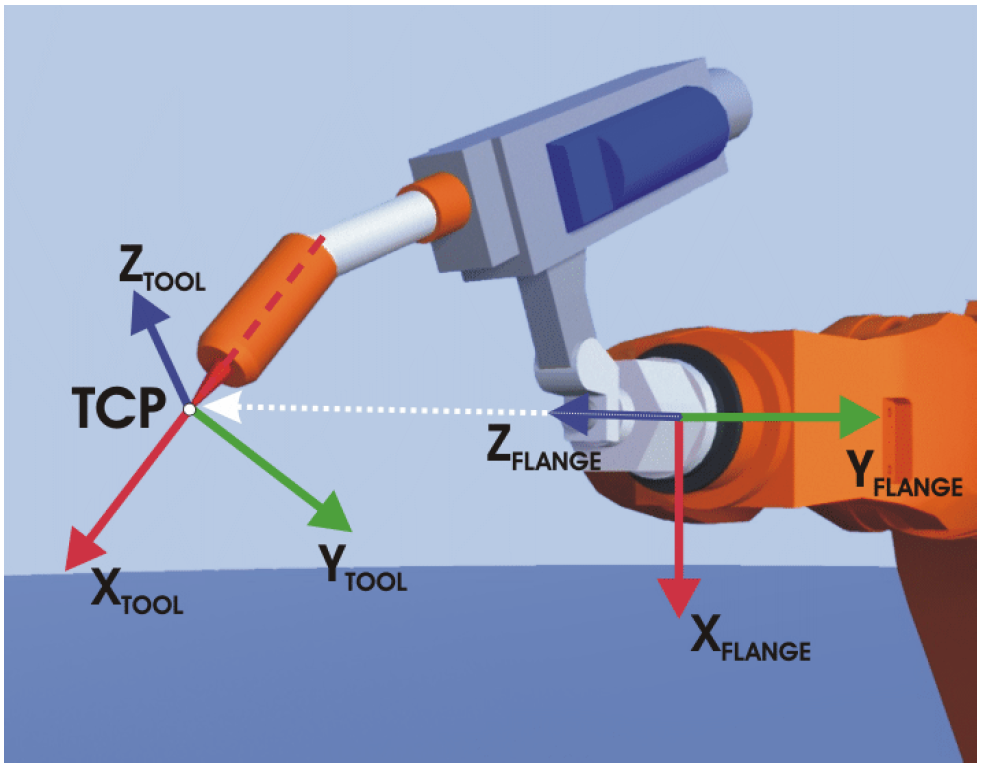
\includegraphics[scale=0.40]{tcp-calibration}
	\caption{A TCP (\angol{Tool Center Point}) elhelyezkedése\cite{sunrisemanual}}
	\label{fig:tcp-calibration}
\end{figure}

Ahhoz hogy egy test pozícióját és orientációját definiálni tudjuk a térben legalább 6 lineárisan független koordinátára van szükség. A viszonyítási koordinátarendszerben felírt 3 transzlációs és 3 rotációs koordináta megfelel erre a célra.
\begin{itemize}
	\item Transzlációs vektorok:
	\begin{itemize}
		\item X távolság: a referencia KR X tengelye mentén vett transzláció
		\item Y távolság: a referencia KR Y tengelye mentén vett transzláció
		\item Z távolság: a referencia KR Z tengelye mentén vett transzláció
	\end{itemize}
	\item Rotációs vektorok:
	\begin{itemize}
		\item A szög: a referencia KR Z tengelye körül vett forgatás
		\item B szög: a referencia KR Y tengelye körül vett forgatás
		\item C szög: a referencia KR X tengelye körül vett forgatás
	\end{itemize}
\end{itemize}

\begin{table}[h]
\setlength\arrayrulewidth{1pt}
\begin{tabu} to\linewidth{| X[1.4,c,m] | X[3,l,m] |}
\hline
\rowfont{\bfseries\large} Koordinátarendszer (KR) & Leírás \\ \hline
Világ KR & A világ KR egy állandó, Descartes-i (Cartesian) koordinátarendszer. Ez minden más KR gyökere, mint például a bázis KR-é vagy a robot bázis KR-é. Alapértelmezetten a világ KR a robot bázispontjában található. \\ \hline
Robot bázis KR & A robot bázis KR-e olyan Descartes-i KR, amely a robotkar bázispontjában található. Ez definiálja a robotkar relatív helyzetét a világ KR-hez képest. Alapértelmezetten a robot bázis KR megegyezik a világ KR-rel. Meg lehet adni egy elforgatási vektort a Sunrise.Workbench-ben, amely definiálja a robot relatív forgatását a világ KR-hez képest. Alapbeállítésként a padlóra rögzített robot felszerelési orientációja: (A=0°, B=0°, C=0°).\\ \hline
Bázis KR & Ahhoz hogy a Descartes-i térben mozgásokat definiálhassunk szükség van referencia KR (bázis) felvételére. Sztenderd módon a világ KR a mozgás bázis KR-e. További bázis KR-eket lehet definiálni a világ KR-hez képest. Ezt mutatja be a FEJEZET HIVATKOZÁS!!!!. \\ \hline
\angol{Flange} KR & A flange KR írja le a robot \angol{flange} középpontjának a pozícióját és orientációját. Ennek az elhelyezkedése nem fix, a robottal együtt mozog. A \angol{flange} KR használható a rá fogatott szerszámokhoz kötődő KR-ek origójaként. Például a szakdolgozat keretében a gripper egy jól definiált pontjára illesztett KR a robot \angol{flange} KR-éhez kepést relatív lett megadva (\ref{fig:tcp-calibration}). \\ \hline
Szerszám KR & A szerszám KR az a Descartes-i KR, amely a felszerelt szerszám munkapontjára illeszkedik. Ezt hívják szerszám középpontnak (\angol{Tool Center Point} - \textbf{TCP}). Bármennyi frame-et lehet definiálni egy szerszámhoz és ezek mindegyike kiválasztható TCP-nek. A szerszám KR rendszerint a \angol{flange} KR-ből származtatott. \\ \hline
\end{tabu}
\caption{A főbb koordinátarendszerek}
\label{tab:coordsystems}
\end{table}

\begin{figure}[h]
	\centering
	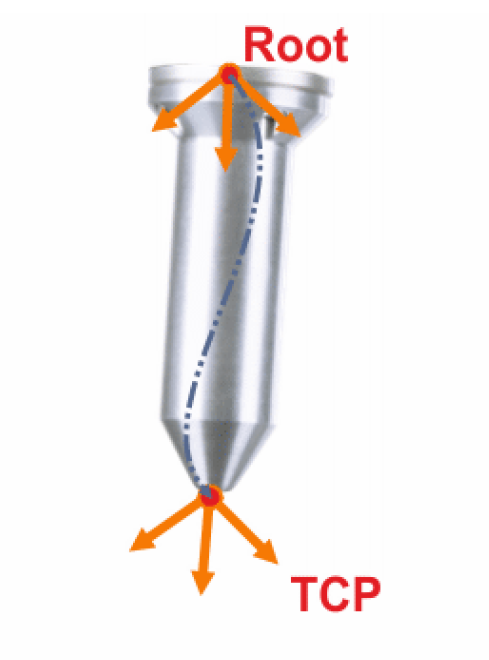
\includegraphics[scale=0.35]{tcp-example1}
	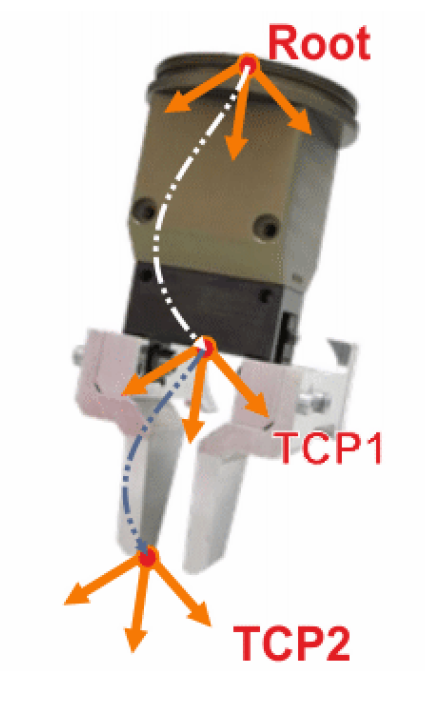
\includegraphics[scale=0.35]{tcp-example2}
	\caption{Szerszám 1 (balra) és 2 (jobbra) TCP-vel\cite{sunrisemanual}}
	\label{fig:tcp-examples}
\end{figure}

\newpage
\subsection{Szerszámkalibráció - XZY 4-pont metódus}
A sakkprojekt kivitelezése során szükséges a robotkarra szerelt megfogó kalibrálása ahhoz, hogy a pozícionálás minél pontosabb legyen. A robotkar szoftverében ez egy alapfunkció, kiegészítő csomag nem szükséges hozzá. A kalibrációs eljárás alapvetően 2 lépésből áll:
\begin{enumerate}
	\item a TCP origójának meghatározásból,
	\item az origóra illesztett koordinátarendszer orientálásából.
\end{enumerate}
A második lépés jelen esetben elhagyható, megfelelő ha a TCP az orientációját a referencia KR-től örökli. 

A TCP origójának meghatározására használt módszer: XYZ 4-pont metódus. Ehhez ki kell választanunk a szerszám egy adott pontját adott helyzetben (pl.: gripper egyik csúcspontja nyitott állásban); ez lesz a TCP. Az eljárás lényege, hogy a kalibrálni kívánt szerszám ezen pontját egy referenciaponthoz vezéreljük 4 különböző irányból. A referencia pont szabadon választható. A robot kontroller a különböző \angol{flange} pozíciókból számolja ki a TCP helyzetét.

A 4 \angol{flange} pozíció egymás közötti távolságainak meg kell haladniuk egy előre definiált minimumot. Ha a pontok túl közel vannak egymáshoz, akkor a pozíció adatokat nem lehet elmenteni. Erre hibaüzenet figyelmeztet.

A kalibráció minősége a transzlációs vektor hibájával mérhető, amit a program kalibráció közben számít ki. Ha ez a hiba meghalad egy definiált határértéket, akkor célszerű a TCP-t újból kalibrálni.

A minimális távolságok és a maximális számítási hiba a \angol{Sunrise Workbench}-ben konfigurálható. Részletesebb leírás az eljárásról a megfelelő Sunrise.OS verzió manuáljában található\cite{sunrisemanual}.

\begin{figure}[h]
	\centering
	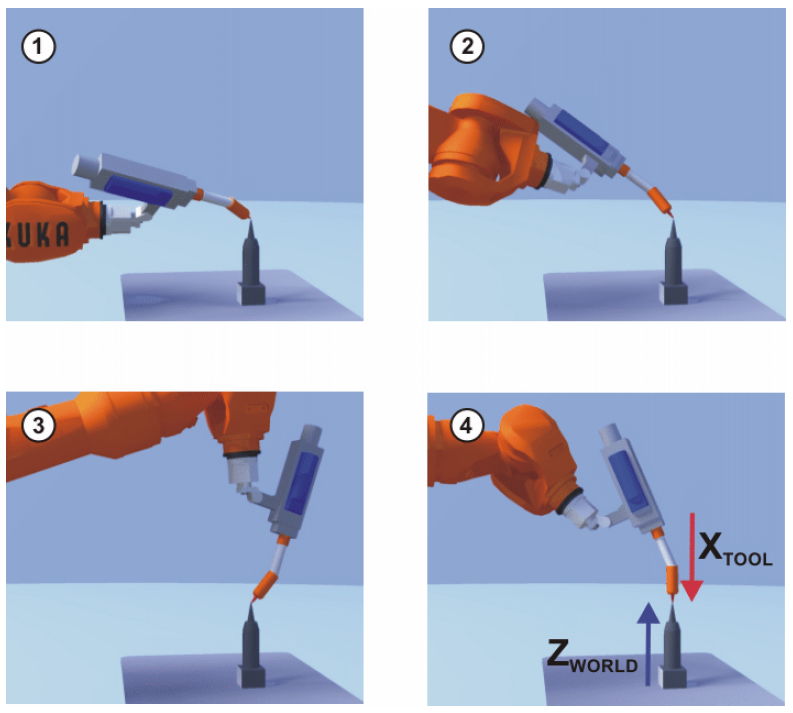
\includegraphics[scale=0.50]{tcp-calibration2}
	\caption{XYZ 4-pont metódus 4 lépése\cite{sunrisemanual}}
	\label{fig:tcp-examples}
\end{figure}

\subsection{Báziskalibráció - 3 pont metódus}
A báziskalibráció során a felhasználó egy Descartes-i koordinátarendszert (bázis koordinátarendszert) rendel a bázisnak választott frame-hez. A bázis KR-nek a felhasználó által választott, tetszőleges helyen lehet az origója.

A bázis kalibráció előnyei:
\begin{enumerate}
	\item A TCP végigvezérelhető a munkafelület szélein vagy egy munkadarabon.
	\item A bázishoz viszonyítva lehet felvenni a szükséges pontokat. Ez a szakdolgozat során azért fontos, mert így nem kell a sakktábla egyes mezőihez tartozó pontokat külön felvenni, a pozíciókat meg lehet adni a bázisponthoz képest, ami lehet például a sakktábla egyik sarokpontja.
\end{enumerate}

A 3-pont metódus során az origó és a bázis 2 további pontja kerül rögzítésre. Az origó felvétele után a kívánt X tengely pozitív felén egy tetszőleges pont rögzítése következik. Végezetül az XY sík első térnegyedébe eső, szintén tetszőlegesen választott pontot kell felvenni. Ez a 3 pont egyértelműen meghatározza a bázist.

A rögzített pontok origótól vett távolságának meg kell haladnia egy minimumot, illetve az egyenesek között is meg kell lennie egy minimum szögnek (origó - X tengely és origó - XY síkon felvett pont). Ha a pontok túl közel vannak vagy az említett szőgek túl kicsik, akkor a pozíció adatokat nem lehet elmenteni. Erre hibaüzenet figyelmeztet.

A minimális távolságok és szögek a \angol{Sunrise Workbench}-ben módosíthatók. Részletesebb leírás az eljárásról a megfelelő Sunrise.OS verzió manuáljában található\cite{sunrisemanual}.

\begin{figure}[h]
	\centering
	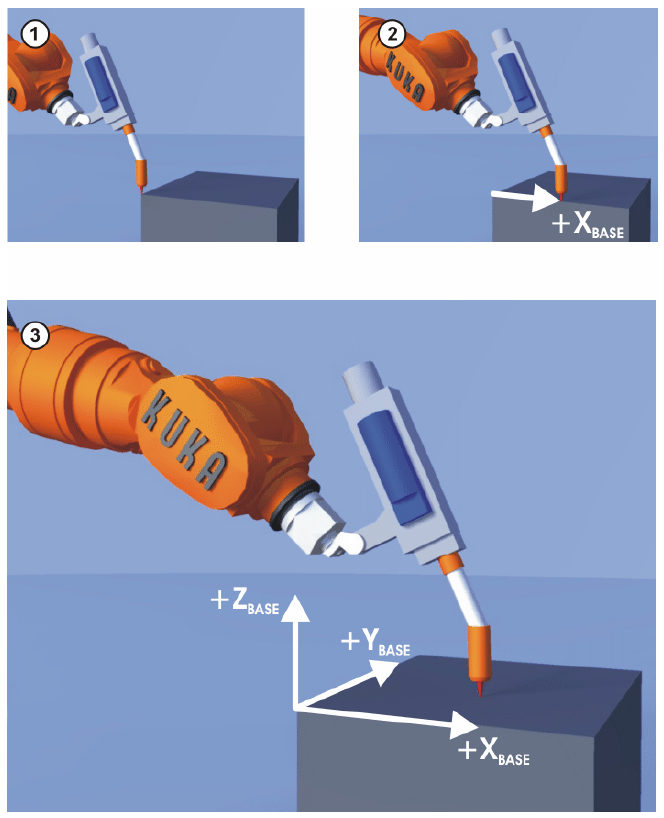
\includegraphics[scale=0.50]{basecalibration}
	\caption{Báziskalibráció 3-pont metódussal\cite{sunrisemanual}}
	\label{fig:basecalibration}
\end{figure}

\subsection{A szerszám tömegeloszlásának meghatározása}
A robotkaron tengelyeiben ébredő többlet nyomatékra meg lehet határozni egy maximális értéket, így ha a munkaterében lévő objektummal ütközik, detektálja és megáll. A robot saját tömegének dinamikus mozgatásához szükséges nyomatéka nem adódik hozzá ehhez a többlet nyomatékhoz. Adott szerszám robotkarra erősítésével viszont előfordulhat, hogy a maximális járulékos nyomatékérték átlépi valamelyik tengelyen a megengedett nyomatékértéket. Ezen hatás korrigálásához szükséges a szerszám tömegeloszlásának kalibrálása (a sakkbábuk, mint munkadarabok kalibrálása nem szükséges, azok tömege elhanyagolható).

A tömegeloszlás meghatározásához a robot először különböző méréseket futtat automatikusan a csuklótengelyek (utolsó három tengely: A5, A6, A7) mozgatásával. Ez alapján a robotkarra szerelt szerszám tömege és a tömegközéppontjának helye meghatározható. Másik lehetőség a szerszám tömegének megadása (például katalógus alapján), majd ez alapján a tömegközéppont helyének kalibrálása.

Az eljárás futtatásához nincs szükség plusz csomagra, a funkció a robotszoftver beépített eleme. A lépések a következők (automatikusan történik, a folyamat 1-2 percet vesz igénybe):
\begin{enumerate}
	\item A folyamat kezdetén az A7 tengelyt a vezérlő a 0 pozícióba mozgatja. Ezen kívül az A5 tengelyt úgy pozícionálja, hogy az A6-os tengelyre többletnyomatékot a súly ne fejtsen ki. Ekkor a szerszám tömegközéppontja abba a síkba esik, amit az A6 tengely és a gravitációs térerősségvektor kifeszít.
	\item A mérés futása során az A6 és az A7 tengelyek egy bizonyos tartományban vesznek fel helyzeteket:
	\begin{itemize}
		\item Alapbeállításként az A6 tengely -95° és +95° közötti vesz fel pozíciókat.
		Ha a munkatér nem elég nagy ehhez a mozgástartományhoz, akkor ez a tartomány csökkenthető.
		\item Az A7 tengely 0°és -90° között mozog.
	\end{itemize}
\end{enumerate}

A mérést befolyásoló tényezőkről információ a Sunrise kézikönyvében\cite{sunrisemanual} található.

\begin{figure}[h]
	\centering
	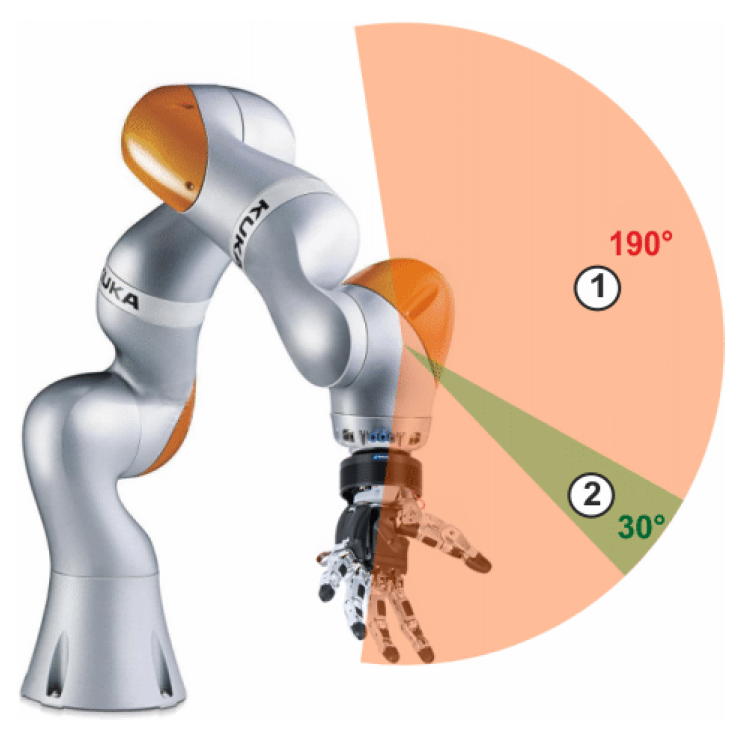
\includegraphics[scale=0.50]{loaddatacalibration}
	\caption{Az A6 tengely mozgástartománya: 1-es esetben teljes, 2-es esetben csökkentett tartomány\cite{sunrisemanual}}
	\label{fig:loaddatacalibration}
\end{figure}

















\end{document}